\documentclass[aspectratio=169,11pt]{beamer}
\usepackage[utf8]{inputenc}
\usepackage[T1]{fontenc}
\usepackage[spanish]{babel}
\usepackage{amsmath,amssymb}
\usepackage{tikz}
\usetikzlibrary{arrows.meta,angles,calc,positioning}
\usetheme{Madrid}
\usecolortheme{default}
\setbeamertemplate{navigation symbols}{}
\setbeamertemplate{blocks}[rounded][shadow=false]
\newcommand{\ang}[1]{\angle #1^\circ}

\title[QFT en Python]{Paso 17: QFT en Python}
\subtitle{Una biblioteca de unas 210 líneas, función por función}
\author{Curso de control robusto (QFT)}
\date{}
\begin{document}
\begin{frame}\titlepage\end{frame}

\begin{frame}{Dónde encaja este paso}
  \tiny
  \begin{enumerate}\setlength{\itemsep}{-2pt}
    \item[1.] Números complejos \hfill \textcolor{gray}{(hecho)}
    \item[2.] Funciones de transferencia: $s$, polos y ceros \hfill \textcolor{gray}{(hecho)}
    \item[3.] Respuesta en frecuencia: $s=j\omega$, magnitud y fase \hfill \textcolor{gray}{(hecho)}
    \item[4.] Decibelios y escala logarítmica (Bode) \hfill \textcolor{gray}{(hecho)}
    \item[5.] Realimentación: $L$, $T=\frac{L}{1+L}$, $S=\frac{1}{1+L}$ \hfill \textcolor{gray}{(hecho)}
    \item[6.] Nichols chart \hfill \textcolor{gray}{(hecho)}
    \item[7.] Incertidumbre y templates \hfill \textcolor{gray}{(hecho)}
    \item[8.] Especificaciones $\rightarrow$ bounds \hfill \textcolor{gray}{(hecho)}
    \item[9.] Loop shaping, prefiltro y verificación \hfill \textcolor{gray}{(hecho)}
    \item[10.] QFT en control digital \hfill \textcolor{gray}{(hecho)}
    \item[11.] Dos caminos digitales: $z$ y $w$ \hfill \textcolor{gray}{(hecho)}
    \item[12.] Estabilidad, límites, más especificaciones y caso real \hfill \textcolor{gray}{(hecho)}
    \item[13.] Muestreo por eventos con periodo base $T$ \hfill \textcolor{gray}{(hecho)}
    \item[14.] Sistemas de dos estados: lazo interno y externo \hfill \textcolor{gray}{(hecho)}
    \item[15.] QFT y sistemas no lineales \hfill \textcolor{gray}{(hecho)}
    \item[16.] Algoritmos de QFT: cómo funcionan por dentro \hfill \textcolor{gray}{(hecho)}
    \item[\textbf{17.}] \textbf{QFT en Python: una biblioteca paso a paso} \hfill $\leftarrow$ estamos aquí
    \item[18.] QFT en MATLAB: el mismo código, otra sintaxis
    \item[19.] Historia, panorama y bibliografía
  \end{enumerate}
  \vspace{2pt}
  \begin{block}{Objetivo de hoy}
    \footnotesize
    Programar los algoritmos del paso 16 en Python con \texttt{numpy} y \texttt{scipy}. Todo el código de las diapositivas es el de \texttt{qftlib.py} (viene en el zip) y \textbf{se ha ejecutado}: las salidas mostradas son las reales.
  \end{block}
\end{frame}

\begin{frame}{Estructura de la biblioteca}
  \small
  \begin{center}
  \begin{tabular}{l|l}
    Función & Hace\\\hline
    \texttt{plant\_family}, \texttt{template} & familia de plantas y $P_i(j\omega)$\\
    \texttt{boundary\_indices} & plantas del borde de la caja de parámetros\\
    \texttt{spec\_stability}, \texttt{spec\_tracking},\\\texttt{spec\_disturbance}, \texttt{spec\_noise} & fabrican una especificación\\
    \texttt{allowed\_map} & mapa de bounds (fase$\times$módulo)\\
    \texttt{margin\_db}, \texttt{check\_L0} & margen de $L_0$ frente a los mapas\\
    \texttt{shape\_de}, \texttt{synthesize\_refine} & loop shaping automático y refinado\\
    \texttt{prefilter\_search}, \texttt{verify} & prefiltro y verificación densa
  \end{tabular}
  \end{center}
  \footnotesize
  \begin{itemize}
    \item Dependencias: \texttt{numpy}, \texttt{scipy} (\texttt{ConvexHull} solo para la comparación y \texttt{differential\_evolution}).
    \item Convenciones: fase en grados en $[-360,0)$, módulo en dB, $\omega$ en rad/s.
    \item Que yo sepa, \texttt{python-control} no incluye QFT: no hay biblioteca estándar, por eso la escribimos.
  \end{itemize}
\end{frame}

\begin{frame}[fragile]{1. Familia y templates}
\footnotesize
La planta es una función de $(\omega,\theta)$; la familia, el producto cartesiano de rejillas de $\theta$.
\footnotesize
\begin{verbatim}
def plant_family(grids):
    """Producto cartesiano de rejillas de parametros -> lista de tuplas theta_i."""
    mesh = np.meshgrid(*grids, indexing="ij")
    return np.stack([m.ravel() for m in mesh], axis=1)
\end{verbatim}

\footnotesize
\begin{verbatim}
def template(Pfun, thetas, w):
    """P_i(jw) para todos los parametros (vector complejo de N elementos)."""
    return np.array([Pfun(w, *th) for th in thetas])
\end{verbatim}
\footnotesize
\begin{verbatim}
def boundary_indices(thetas):
    """Plantas con ALGUN parametro en un extremo de su rango (borde de la caja).
    Para estas especificaciones da el mismo mapa que usar toda la familia."""
    lo, hi = thetas.min(0), thetas.max(0)
    return np.where(((thetas == lo) | (thetas == hi)).any(axis=1))[0]
\end{verbatim}
\scriptsize Con \texttt{grids = [linspace(1,5,17), linspace(1,3,13)]} se obtienen 221 filas $(K,a)$; \texttt{boundary\_indices} devuelve 56.
\end{frame}

\begin{frame}[fragile]{2. Especificaciones como funciones}
\footnotesize
Una especificación es una función \texttt{f(L, w)} que recibe $L_i$ de todas las plantas y devuelve \texttt{True} si se cumple. Se crean con una \emph{clausura}:
\footnotesize
\begin{verbatim}
def spec_stability(Ws):
    """|L/(1+L)| <= Ws  para todas las plantas."""
    return lambda L, w: np.all(np.abs(L / (1 + L)) <= Ws, axis=-1)
\end{verbatim}
\footnotesize
\begin{verbatim}
def spec_tracking(delta_db):
    """dispersion de |T_i| en dB <= delta_db(w): el prefiltro hara el resto."""
    def f(L, w):
        t = 20 * np.log10(np.abs(L / (1 + L)))
        return (t.max(-1) - t.min(-1)) <= delta_db(w)
    return f
\end{verbatim}
\footnotesize
\begin{verbatim}
def spec_disturbance(Wd):
    """|1/(1+L)| <= Wd(w)  (rechazo de perturbacion a la salida)."""
    return lambda L, w: np.all(1 / np.abs(1 + L) <= Wd(w), axis=-1)
\end{verbatim}
\scriptsize Las matrices \texttt{L} tienen forma \texttt{[n\_fase, n\_modulo, n\_plantas]}; \texttt{axis=-1} reduce sobre las plantas.
\end{frame}

\begin{frame}[fragile]{3. El mapa de bounds}
\scriptsize
\begin{verbatim}
def allowed_map(w, ratios, specs, idx=None, ph=PH, mg=MG):
    """Mapa booleano [len(ph), len(mg)]: True si L0 (fase ph, modulo mg dB)
    cumple TODAS las specs para las plantas del template (r_i = P_i / P_0).
    idx: subconjunto de plantas (None = todas)."""
    r = ratios if idx is None else ratios[idx]
    L0 = 10 ** (mg[None, :] / 20) * np.exp(1j * np.radians(ph)[:, None])
    L = L0[..., None] * r                      # forma [nph, nmg, N]
    ok = np.ones(L0.shape, bool)
    for s in specs:
        ok &= s(L, w)
    return ok
\end{verbatim}

\footnotesize
\begin{itemize}
\item \texttt{L0} es $360\times241$; \texttt{L0[..., None] * r} la expande a $360\times241\times N$ (\emph{broadcasting}).
\item Memoria: con $N=56$ son $4.9$ millones de complejos, unos 78 MB por matriz; con 221, unos 307 MB.
\item \texttt{ok \&= s(L, w)} es la intersección de especificaciones.
\end{itemize}
\end{frame}

\begin{frame}[fragile]{4. Margen y comprobación de $L_0$}
\scriptsize
\begin{verbatim}
def wrap_phase(L):
    p = np.degrees(np.angle(L))
    return np.where(p > 0, p - 360, p)
\end{verbatim}
\scriptsize
\begin{verbatim}
def margin_db(okmap, phase, gain_db, ph=PH, mg=MG):
    """Distancia vertical (dB) al borde del mapa: >0 permitido, <0 prohibido."""
    dph = np.abs(((phase - ph + 180) % 360) - 180)   # diferencia en modulo 360
    i = int(np.argmin(dph))
    col = okmap[i]; j = int(np.argmin(np.abs(mg - gain_db)))
    bad = ~col if col[j] else col              # celdas del tipo contrario
    if not bad.any():
        return 60.0 if col[j] else -60.0
    d = np.abs(mg[bad] - gain_db).min()
    return d if col[j] else -d
\end{verbatim}
\scriptsize
\begin{verbatim}
def check_L0(L0fun, wlist, maps):
    """Margen (dB) de L0 frente a los mapas, frecuencia a frecuencia."""
    out = []
    for w, m in zip(wlist, maps):
        L = L0fun(w); out.append(margin_db(m, wrap_phase(L), 20 * np.log10(abs(L))))
    return np.array(out)
\end{verbatim}
\scriptsize \texttt{((phase - ph + 180) \% 360) - 180} mide la diferencia de fase en módulo 360: \texttt{-359} y \texttt{+1} caen en la misma columna.
\end{frame}

\begin{frame}[fragile]{5. Ejemplo completo: el diseño del paso 9}
\scriptsize
\begin{verbatim}
import numpy as np
import qftlib as q
P = lambda w, K, a: K / (1j * w * (1j * w + a))            # planta K/(s(s+a))
grids = [np.linspace(1, 5, 17), np.linspace(1, 3, 13)]    # K, a  -> 221 plantas
thetas = q.plant_family(grids)
Ws = 1.2
TU = lambda w: abs(1 / ((1j * w / 8) ** 2 + 2 * 0.6 * (1j * w / 8) + 1))
TL = lambda w: abs(1 / (1j * w / 1.2 + 1) ** 3)
delta_db = lambda w: 20 * np.log10(TU(w) / TL(w))
Wd = lambda w: 0.3 if w <= 0.5 else (0.5 if w <= 1.0 else 10.0)
specs = [q.spec_stability(Ws), q.spec_tracking(delta_db), q.spec_disturbance(Wd)]
wlist = [0.1, 0.5, 1, 2, 5, 10, 20, 50]
idx = q.boundary_indices(thetas)                          # 56 plantas del borde
maps = []
for w in wlist:
    z = q.template(P, thetas, w)
    r = z / P(w, 1.0, 1.0)                                # nominal: K=1, a=1
    maps.append(q.allowed_map(w, r, specs, idx=idx))
G9 = lambda s: 5 * (1 + s / 2) / (1 + s / 20)
L0 = lambda w: G9(1j * w) * P(w, 1.0, 1.0)
print("margenes (dB):", np.round(q.check_L0(L0, wlist, maps), 2))
\end{verbatim}
\end{frame}

\begin{frame}[fragile]{Salida real}
  \footnotesize
  \begin{verbatim}
margenes (dB): [ 6.45  0.79  0.93 17.94 60.   60.    5.54 16.12]
verificacion densa G9: 0 frecuencias fallan
  \end{verbatim}
  \begin{itemize}
    \item Los márgenes son positivos en las ocho frecuencias: $G(s)=5\frac{1+s/2}{1+s/20}$ cumple los bounds. El mínimo es $0.79$ dB, en $\omega=0.5$.
    \item $60$ significa ``sin celdas prohibidas en esa fase'' (valor truncado).
    \item La verificación densa (221 plantas, 400 frecuencias) \textbf{no encuentra fallos}: el código reproduce el resultado del paso 9.
  \end{itemize}
  \begin{alertblock}{Cómo se sabe que el código es correcto}
    Tres pruebas (siguiente diapositiva): borde frente a toda la familia, la fórmula cerrada del paso 16 y la verificación densa.
  \end{alertblock}
\end{frame}

\begin{frame}[fragile]{6. Loop shaping automático}
\scriptsize
\begin{verbatim}
def shape_de(P0fun, wlist, maps, bounds=((0.5, 30), (0.2, 20), (2, 200)),
             seed=1, maxiter=60):
    """Busca (k, z, p) que cumple los mapas con el menor G(inf) = k p / z
    (menos ruido en alta frecuencia)."""
    def cost(x):
        k, z, p = x
        G = lambda s: k * (1 + s / z) / (1 + s / p)
        m = check_L0(lambda w: G(1j * w) * P0fun(w), wlist, maps)
        pen = np.sum(np.clip(-m, 0, None))                       # dB de violacion
        return k * p / z + 1e3 * pen
    r = differential_evolution(cost, bounds, seed=seed, maxiter=maxiter,
                               tol=1e-6, polish=False)
    return r.x, r.fun
\end{verbatim}

\footnotesize
\begin{itemize}
\item \texttt{cost} devuelve $G(\infty)=kp/z$ más $10^3\times$ los dB de violación.
\item \texttt{differential\_evolution} evalúa unas 1000--2000 veces \texttt{cost}; cada una recorre las $\omega$ de \texttt{wlist}.
\item \texttt{seed} fija el resultado: sin semilla cambia en cada ejecución.
\end{itemize}
\end{frame}

\begin{frame}[fragile]{7. El bucle de refinado}
\scriptsize
\begin{verbatim}
def synthesize_refine(P0fun, Pfam, specs, wlist, wdense, make_map,
                      bounds=((0.5, 30), (0.2, 20), (2, 200)), iters=8, add=3):
    """Bucle de refinado: DE con los mapas actuales -> verificacion densa
    -> anadir frecuencias que fallan -> repetir.
    make_map(w) -> mapa permitido a la frecuencia w.  Devuelve (x, historial)."""
    wl = list(wlist); maps = [make_map(w) for w in wl]; hist = []
    for it in range(iters):
        x, f = shape_de(P0fun, wl, maps, bounds)
        G = lambda s, x=x: x[0] * (1 + s / x[1]) / (1 + s / x[2])
        bad = verify(lambda w: G(1j * w) * Pfam(w), wdense, specs)
        hist.append((x.copy(), x[0] * x[2] / x[1], len(bad), len(wl)))
        if len(bad) == 0:
            break
        pos = np.linspace(0, len(bad) - 1, min(add, len(bad))).astype(int)
        new = bad[pos]                                   # fallos repartidos
        for w in new:
            wl.append(float(w)); maps.append(make_map(w))
    return x, hist
\end{verbatim}
\end{frame}

\begin{frame}{Resultado del refinado (Python)}
  \footnotesize
  \centering
  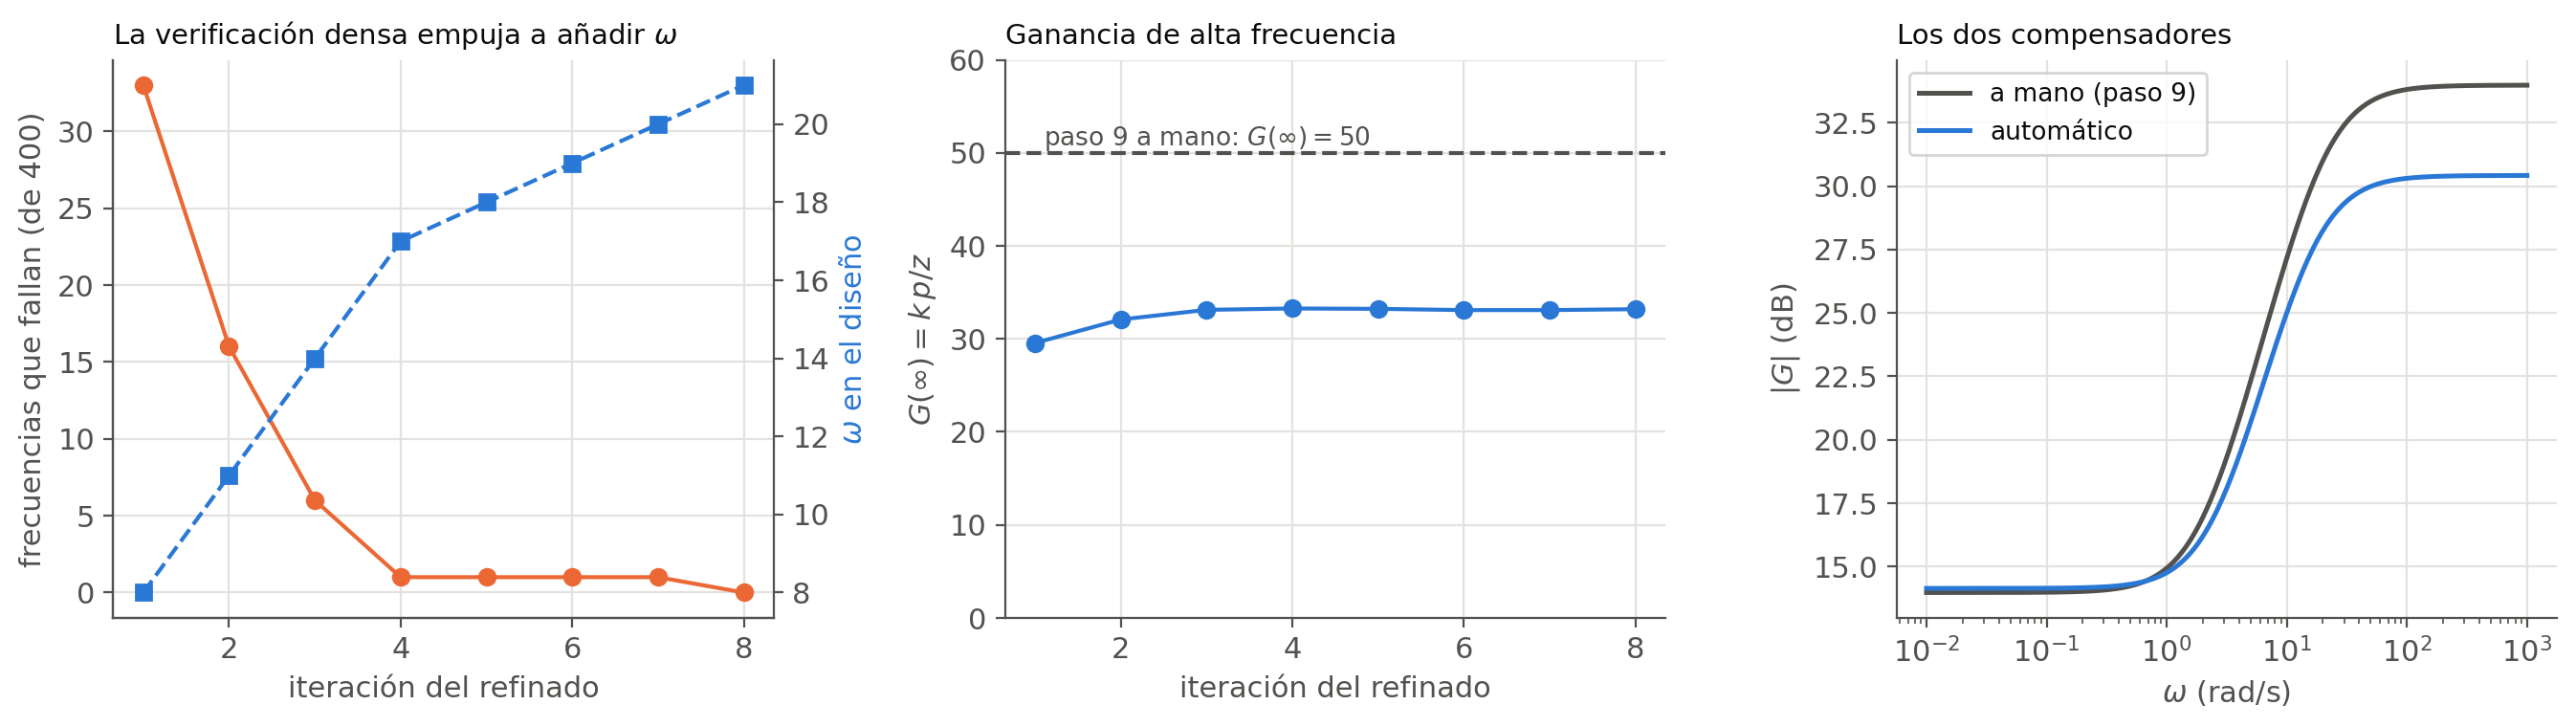
\includegraphics[width=\textwidth]{fig/refinado.png}\\[2pt]
  \begin{itemize}
    \item Ocho iteraciones, 21 frecuencias en el diseño final y $16.5$ s de cálculo.
    \item Diseño final: $k=5.095$, $z=2.521$, $p=16.43$, $G(\infty)=33.2$, \textbf{0 fallos} en la verificación densa. Frente a $50$ del diseño a mano.
    \item Las iteraciones 4 a 7 siguen con 1 fallo: añadir frecuencias \textbf{no} garantiza converger en una vuelta; el bucle insiste hasta que pasa.
  \end{itemize}
\end{frame}

\begin{frame}[fragile]{8a. Prefiltro}
\scriptsize
\begin{verbatim}
def prefilter_search(Tfam, TUf, TLf, W, fgrid):
    """Elige el polo f de F = 1/(1+s/f): maximiza el margen minimo (dB)
    dentro de la banda [T_L, T_U].
    Tfam(w) -> |T_i(jw)| de todas las plantas; TUf, TLf -> |T_U|, |T_L|."""
    best = (-1e9, None)
    for f in fgrid:
        m = 1e9
        for w in W:
            t = Tfam(w) / abs(1 + 1j * w / f)
            m = min(m, 20 * np.log10(TUf(w) / t.max()),
                       20 * np.log10(t.min() / TLf(w)))
        if m > best[0]:
            best = (m, f)
    return best          # (margen dB, f)
\end{verbatim}
\footnotesize Con $G$ del paso 9: \texttt{f = 1.1}, margen $0.028$ dB. Con el $G$ automático: \texttt{f = 1.0}, $0.032$ dB.
\end{frame}

\begin{frame}[fragile]{8b. Verificación densa}
\scriptsize
\begin{verbatim}
def verify(Lfam, wdense, specs):
    """Comprueba las specs en TODAS las plantas y frecuencias; devuelve las
    frecuencias que fallan.
    Lfam(w) -> L_i(jw) de la familia (vector)."""
    bad = []
    for w in wdense:
        L = Lfam(w)
        if not all(bool(s(L[None, :], w)[0]) for s in specs):
            bad.append(w)
    return np.array(bad)
\end{verbatim}
\footnotesize Recorre 400 frecuencias y devuelve las que fallan: es la entrada del bucle de refinado. \texttt{s(L[None, :], w)[0]} aprovecha que cada especificación espera una matriz 3D.
\end{frame}

\begin{frame}[fragile]{9a. Bounds exactos: las cuadráticas}
\scriptsize
\begin{verbatim}
def quad_stability(ws):                          # |T| <= ws, una planta
    return lambda u: ((ws**2 - 1) * abs(u)**2, 2 * ws**2 * u.real, ws**2 + 0 * u.real)
\end{verbatim}
\scriptsize
\begin{verbatim}
def quad_disturbance(wd):                        # |S| <= wd, una planta
    return lambda u: (abs(u)**2, 2 * u.real, 1 - 1 / wd**2 + 0 * u.real)
\end{verbatim}
\scriptsize
\begin{verbatim}
def quad_tracking_pairs(R):                      # |T_d| / |T_e| <= R, para cada par (d, e)
    def f(u):
        ud, ue = np.meshgrid(u, u, indexing="ij"); m = ~np.eye(len(u), dtype=bool)
        ud, ue = ud[m], ue[m]
        return (abs(ud)**2 * abs(ue)**2 * (R**2 - 1),
                2 * (R**2 * abs(ue)**2 * ud.real - abs(ud)**2 * ue.real),
                R**2 * abs(ue)**2 - abs(ud)**2)
    return f
\end{verbatim}
\footnotesize Cada función devuelve $(a,b,c)$ para $a x^2+bx+c\ge0$ con $x=|L_0|$. El seguimiento recorre los $N(N-1)$ pares con \texttt{meshgrid}.
\end{frame}

\begin{frame}[fragile]{9b. Bounds exactos: intervalos prohibidos}
\scriptsize
\begin{verbatim}
def forbidden_intervals(a, b, c):
    """Intervalos (lo, hi) de x > 0 donde a x^2 + b x + c < 0, para vectores a, b, c."""
    lo, hi = [], []
    D = b**2 - 4 * a * c
    with np.errstate(all="ignore"):
        s = np.sqrt(np.where(D > 0, D, 0.0))
        r1, r2 = (-b - s) / (2 * a), (-b + s) / (2 * a)
        xa, xb = np.minimum(r1, r2), np.maximum(r1, r2)
        pos = (a > 1e-12) & (D > 0)               # parabola hacia arriba: prohibido entre raices
        neg = a < -1e-12                          # hacia abajo: prohibido fuera de las raices
        lo += [xa[pos]]; hi += [xb[pos]]
        both = neg & (D > 0)
        lo += [np.zeros(both.sum()), xb[both]]; hi += [xa[both], np.full(both.sum(), np.inf)]
        allx = neg & (D <= 0)
        lo += [np.zeros(allx.sum())]; hi += [np.full(allx.sum(), np.inf)]
    lo, hi = np.concatenate(lo), np.concatenate(hi)
    ok = hi > np.maximum(lo, 0)
    return np.maximum(lo[ok], 0.0), hi[ok]
\end{verbatim}
\footnotesize Resuelve $a x^2+bx+c<0$ para vectores: parábola hacia arriba, prohibido entre raíces; hacia abajo, fuera de ellas.
\end{frame}

\begin{frame}[fragile]{9c. Bounds exactos: unión de intervalos}
\scriptsize
\begin{verbatim}
def exact_forbidden(ratios_edge, phase_deg, quads):
    """Union (ordenada) de intervalos prohibidos de |L0| (en dB) para una fase concreta."""
    u = ratios_edge * np.exp(1j * np.radians(phase_deg))
    los, his = [], []
    for qd in quads:
        lo, hi = forbidden_intervals(*qd(u)); los.append(lo); his.append(hi)
    lo, hi = np.concatenate(los), np.concatenate(his)
    if lo.size == 0:
        return np.empty((0, 2))
    o = np.argsort(lo); lo, hi = lo[o], hi[o]
    reach = np.maximum.accumulate(hi)
    start = np.r_[True, lo[1:] > reach[:-1]]
    ends = np.r_[start[1:], True]
    L = 20 * np.log10(np.maximum(lo[start], 1e-12)); H = 20 * np.log10(reach[ends])
    return np.column_stack([L, H])
\end{verbatim}
\footnotesize Unión: ordenar por extremo inferior y acumular el máximo.
\end{frame}

\begin{frame}[fragile]{9d. Bounds exactos: margen}
\scriptsize
\begin{verbatim}
def exact_margin_db(ratios_edge, phase_deg, gain_db, quads):
    """Margen vertical exacto (dB) de L0 a la frontera: >0 si esta permitido."""
    iv = exact_forbidden(ratios_edge, phase_deg, quads)
    inside = (iv[:, 0] <= gain_db) & (gain_db <= iv[:, 1]) if len(iv) else np.array([], bool)
    d = np.min(np.minimum(abs(iv[:, 0] - gain_db), abs(iv[:, 1] - gain_db))) if len(iv) else 60.0
    return -d if inside.any() else d
\end{verbatim}
\footnotesize Distancia vertical en dB al extremo más cercano; negativa si $L_0$ está dentro de un intervalo prohibido; $60$ dB si no hay ninguno.
\end{frame}

\begin{frame}[fragile]{Pruebas (test\_qft.py)}
  \footnotesize
  \begin{verbatim}
w=  0.1: borde    0 celdas erroneas | hull   21
w=    1: borde    0 celdas erroneas | hull    3
w=    2: borde    0 celdas erroneas | hull  263
w=    5: borde    0 celdas erroneas | hull  261
w=   20: borde    0 celdas erroneas | hull  260
w=1.0: formula cerrada vs rejilla, celdas distintas = 0
w=2.0: formula cerrada vs rejilla, celdas distintas = 0
verificacion densa: frecuencias que fallan = 0
w=0.5: exacto vs rejilla, celdas distintas = 0; margen exacto = 0.701 dB
w=1.0: exacto vs rejilla, celdas distintas = 0; margen exacto = 0.627 dB
w=2.0: exacto vs rejilla, celdas distintas = 0; margen exacto = 17.673 dB
  \end{verbatim}
  \begin{itemize}
    \item \textbf{Prueba 1}: el borde de la caja da el mismo mapa que toda la familia; la envolvente convexa, no.
    \item \textbf{Prueba 2}: la fórmula cerrada del bound de estabilidad coincide con la rejilla en las $86\,760$ celdas.
    \item \textbf{Prueba 3}: el diseño del paso 9 pasa la verificación densa.
    \item \textbf{Prueba 4}: los bounds exactos coinciden con la rejilla (0 celdas distintas) y dan el margen real.
  \end{itemize}
  \scriptsize Si cambias la rejilla o la especificación, estas cuatro pruebas dicen si algo se rompió.
\end{frame}

\begin{frame}{Rendimiento y cómo acelerarlo}
  \small
  \begin{itemize}
    \item Un mapa con 56 plantas tarda unos $0.23$ s; ocho mapas, unos 2 s; la búsqueda de refinado, $16.5$ s en total (la mayor parte es \texttt{verify}, que no está vectorizada).
    \item \textbf{Menos memoria}: procesar la fase por bloques de 30--60 filas; usar \texttt{complex64}.
    \item \textbf{Menos cálculo}: reducir la rejilla de módulo a $1$ dB \textbf{con cuidado} (el margen puede cambiar en $\sim1$ dB, paso 16); pasar a fase $2^\circ$ no cambia nada en este ejemplo.
    \item \textbf{Más rápido}: \texttt{numba} sobre los bucles o vectorizar \texttt{verify} sobre $\omega$.
    \item \textbf{Paralelo}: los mapas de distintas $\omega$ son independientes (\texttt{multiprocessing}).
  \end{itemize}
  \begin{alertblock}{No optimizar a ciegas}
    Medir primero (\texttt{time.time()} o \texttt{cProfile}) y comprobar con las tres pruebas \textbf{después} de cada cambio.
  \end{alertblock}
\end{frame}

\begin{frame}{Cómo extenderlo}
  \small
  \begin{itemize}
    \item \textbf{Más especificaciones}: añadir una función \texttt{spec\_...} y pasarla en la lista \texttt{specs}. Ejemplo: \texttt{spec\_noise(-10)} para el ruido del paso 12.
    \item \textbf{Discreto}: pasar \texttt{P(w, ...)} evaluada en $w=j\nu$ (paso 11) y una lista de $\omega$ hasta Nyquist; el resto no cambia.
    \item \textbf{Otra forma de $G$}: cambiar la lambda de \texttt{shape\_de} (añadir un segundo cero, un integrador).
    \item \textbf{Prefiltro de segundo orden}: ampliar \texttt{prefilter\_search} a dos parámetros.
    \item \textbf{Plantas no paramétricas}: cada planta del template es un punto medido; \texttt{template} puede leer datos en vez de una fórmula.
  \end{itemize}
  \begin{block}{Limitaciones}
    Solo SISO; sin estabilidad por Nyquist para plantas inestables (paso 12): se comprueban los polos a mano; el óptimo de $G(\infty)$ es local.
  \end{block}
\end{frame}

\begin{frame}{Resumen}
  \small
  \begin{itemize}
    \item La biblioteca son $\sim210$ líneas: una función por algoritmo, especificaciones como clausuras, mapas con \emph{broadcasting} 3D.
    \item Reproduce el paso 9 y pasa tres pruebas independientes.
    \item El refinado automático llega a $G(\infty)=33.2$ ($k=5.095$, $z=2.521$, $p=16.43$) con 0 fallos densos.
    \item Cuidado con: memoria (78--307 MB), semilla, y el bucle de refinado (no basta una pasada).
  \end{itemize}
  \begin{block}{Ejercicio}
    (1) Añade \texttt{spec\_noise(-10)} en $\omega\ge30$ y comprueba si el diseño del paso 9 sigue pasando. (2) ¿Qué cambia en \texttt{template} para medir la planta en vez de usar una fórmula? (3) ¿Qué pasa con la memoria si pasas a 1000 plantas?
  \end{block}
\end{frame}

\appendix
\begin{frame}{Solución del ejercicio}
  \footnotesize
  \textbf{1.} Con $G(s)=5\frac{1+s/2}{1+s/20}$, $|T|$ en $\omega=30$ es del orden de $-10$ dB: la especificación del paso 12 exigía el rediseño porque $|T|\le-10$ dB \textbf{y} $|GS|\le60$ juntas. Se prueba añadiendo \texttt{q.spec\_noise(-10)} a \texttt{specs} para $\omega\ge30$ y repitiendo \texttt{verify}.\\[3pt]
  \textbf{2.} \texttt{template} deja de llamar a \texttt{Pfun} y devuelve las respuestas medidas a esa $\omega$ (un vector complejo por experimento); \texttt{boundary\_indices} se sustituye por todos los puntos o por su envolvente (sin la garantía del borde).\\[3pt]
  \textbf{3.} Con 1000 plantas la matriz 3D pasa de 78 MB (56 plantas) a $360\cdot241\cdot1000\cdot16\approx1.4$ GB. Hay que procesar por bloques de fase.
\end{frame}
\end{document}
